
\section{Brick-parametric design}\label{sec:filter}

\subsection{Brick decomposition}\label{sec:brick-decomposition}

Let us assume that medical devices produce 3D images with lateral dimensions that are integer multiples of some powers of two, like 128, 256, 512, etc.
Any cuboidal portion of the image is completely determined by the Cartesian indices of its voxels of lowest and highest indices and extracted by multidimensional array \emph{slicing} as $image([\ell_x : h_x, \ell_y : h_y, \ell_z : h_z])$.

For the sake of simplicity, we assume a common size on the three image axes, and the corresponding image portion $\B$, called \emph{brick}, as a function of its element of the  lowest  brick coordinates $i,j,k\in [1:n]$ and the brick lateral size $n\in\N$:
\[
\B(i,j,k,n) := image([in:in+n, jn:jn+n, kn:kn+n]) 
\]

\begin{figure}[htbp] %  figure placement: here, top, bottom, or page
    \centering
    \begin{subfigure}{0.49\textwidth}
       \centering
       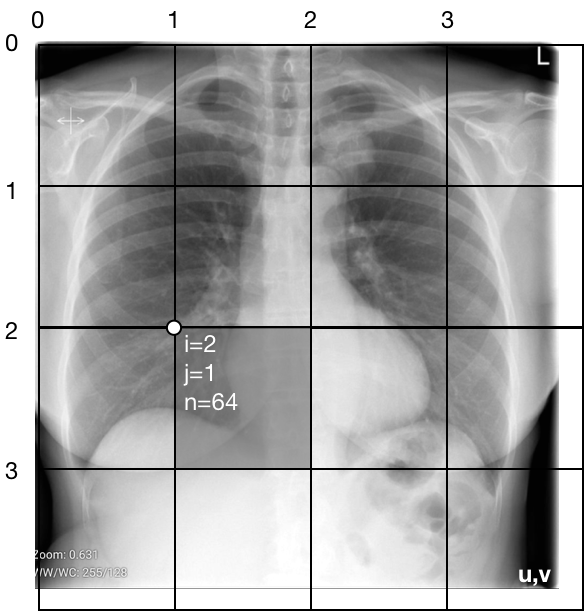
\includegraphics[width=0.70\linewidth]{src/figs/blocks.png} 
       \subcaption{A possible brick partitioning of a radiologic image. The evidenced 2D brick, of size $n^d=64^2$, is sliced by $\B([2,1,64]) = Image([128:172],[64:128)]$}
       \label{fig:bricks}
    \end{subfigure} 
    \begin{subfigure}{0.49\textwidth}
        \centering
        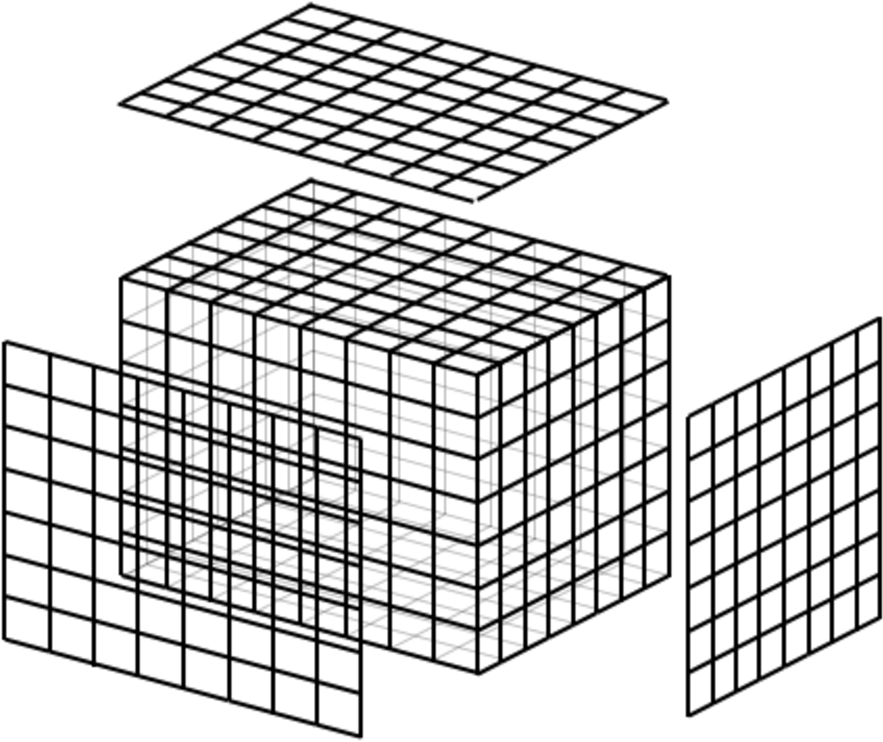
\includegraphics[width=0.99\linewidth]{figs/grid.pdf} 
        \subcaption{Faces on the brick boundary}
        \label{fig:brickboundary}
    \end{subfigure} 
    \caption{Brick decomposition}
\end{figure}


Figure~\ref{fig:bricks} shows the brick decomposition in a 2D image, with positive integers $(u,v)$ giving the lateral sizes of image. Note that brick sides do not necessarily correspond to image edges. 


\subsection{Brick operator }\label{sec:brick}

\subsubsection*{Chain coordinates }\label{sec:chain-coords}
We are going to treat each image brick independently from each other. Hence we map each image brick $\B(i,j,k,n)$ to the linear \emph{chain} space $C_2$ of dimension $n\times n\times n$, using coordinate vectors $c\in \mathbf{2}^{n^d} := \{0,1\}^{n^d}$, where the basis element $c \in C_2$ is mapped via Cartesian-to-linear map to the binary vector 
\[
Image(h,k) \mapsto c_{h,k} := [0 \cdots 0\ 1\ 0 \cdots 0] \in \B^{n\times n}
\]
for each $0\leq h,k \leq n$, and where the (single) unit element is in position $nk + h \leq n\times n$.

Therefore, each pixel (or voxel) in a brick image will be seen as a basis binary vector in $C_2$, and each subset of image elements, as the corresponding binary vector in $C_2$, with many ones as the cardinality of the subset.

\subsubsection*{Boundary operator }\label{sec:boundary-operator}
For a fixed brick size $n$, the boundary operator $\partial_d : C_d\to C_{d-1}$, with $d\in\{2,3\}$, will be constructed once and for all using the algorithm given in~
\cite{TSAS}, 
% \cite{DiCarlo2014}, 
and inlined in the generated boundary extraction code.

It is easy to see that the operator's matrix $[\partial_d]$ is \emph{very sparse}, since it contains $2\times d$ non-zero elements (ones) for each column (of length $n^d$), i.e.~4 ones and 6 ones for the 2D and 3D case, respectively. In fact the matrix of a linear operator between linear spaces contains by columns the basis element of the domain space, represented in the target space. In our case, the former is an image element (2-cube or 3-cube), represented as the chain of its boundary---i.e. either a 1-cycle of 4 edges, or  a 2-cycle of 6 faces, respectively.  

The number of rows of $[\partial_d]$ equates the dimension of the linear space $C_{d-1}$, i.e.~the number of $(d-1)$-cells---elementary $(d-1)$-chains---in the cellular partition of the image. To compute their number, we act in two steps. (a) First we map one-to-one the $n^d$ $d$-cells with $d$ adjacent $(d-1)$-cells, so getting $d\,n^d$ distinct basis elements of $C_{d-1}$. (b) Then we complete this bases by adjoining $n^{d-1}$ boundary elements for each of the $d$ dimensions of the image, so providing further $d\,n^{d-1}$ basis elements for $C_{d-1}$. The dimension of $C_{d-1}$, and therefore the number of rows of $[\partial_d]$ matrix is $d\,(n^{d-1}+n^{d}) = d\,n\,(1+n)^{d-1}$. The number of column equates the number of basis elements of $C_d$, i.e.~the number $n^d$ of brick elements.

\subsubsection*{Sparsity and size of boundary matrix }\label{sec:bm-size}

As we have seen, we have $2d$ non-zero elements for each column of $[\partial_d]$, so that their total number is $2d\,n^d$. The number of matrix element is $d\,n\,(1+n)^{d-1} \times n^d$, giving a ratio of 
\[
\frac{\mbox{non-zero\ elements}}{\mbox{total\ elements}} = 
\frac{2d\times n^d}{d\,n\,(1+n)^{d-1} \times n^d} =
\frac{2}{n+n^d}
\]
Using sparse matrices in CSC (Compressed Sparse Column) format we get a storage size:
\[
mem([\partial_d]_{n^d}) = 2\times \#\mbox{nzero} + \#\mbox{columns} = 2\times 2d\,n^d + n^d = (4d+1)n^d.
\]
In conclusion, for brick size $n=64$, the matrix $[\partial_d]$ requires for 2D images $9\times 64^2=36,864$ memory elements, and for 3D images $13\times 64^3=3,407,872$ memory elements. Counting the bytes for the standard implementation of a sparse binary matrix (1 byte for values and 8 bytes for indices) we get $(18d+8)n^d$ bytes, giving $176$\,KB for 2D and $15.872$\,MB for 3D.


% \begin{figure}[htbp] %  figure placement: here, top, bottom, or page
%   \centering
%   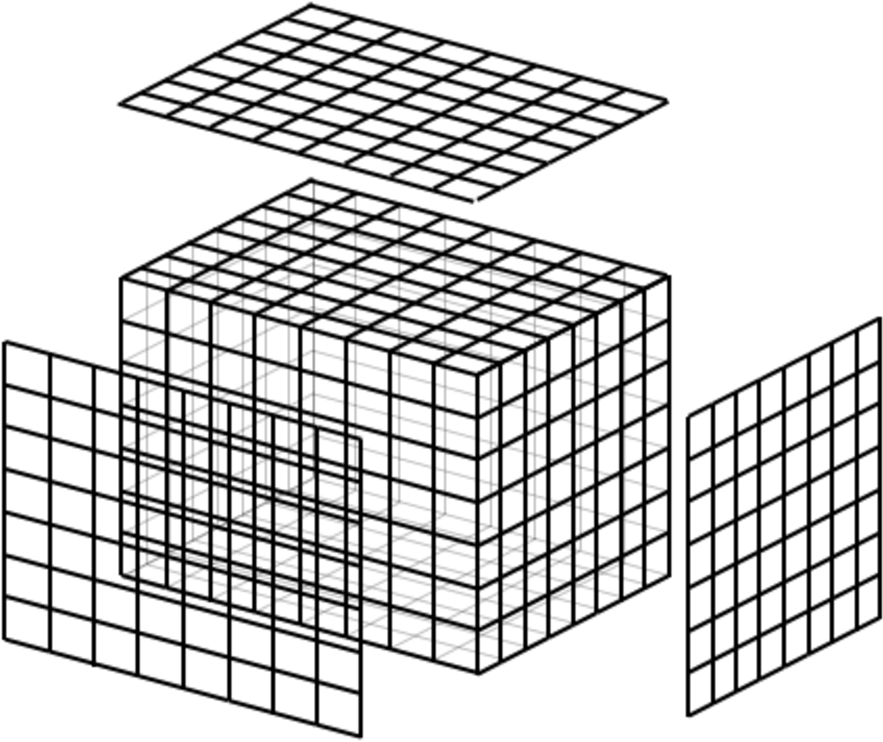
\includegraphics[width=0.4\linewidth]{figs/grid.pdf} 
%   \caption{Faces on the brick boundary}
%   \label{fig:brickboundary}
% \end{figure}



\subsection{Brick boundary mapping}\label{sec:brick-mapping}

Here we refer directly to the 3D case.
Let us call \emph{segment} the bulk content $S$ of interest within the input 3D image of size $(u,v,w)$. Our aim is to compute the segment boundary $\partial_3 S$. 
First we set the size $n$ of the brick, in order to decompose the input $Image(u,v,w)$ into a fair number of bricks
\[
M = \ceil{u/n} \times \ceil{v/n} \times \ceil{w/n} \simeq \frac{uvw}{n^3}.
\] 
Then, we consider each segment portion $c_{i,j,k} = S\cap \B(i,j,k,n)$ and compute its local coordinate representation  $[c]_{i,j,k}\in C_3(n,n,n)$. This one is a sparse binary vector of length $n^3$. Then, assemble the $M$ representations $c$ of segment portions into a sparse binary matrix $\T{S}$, of dimension $n^d \times M$, with $d=3$. Finally, compute a matrix $\T{\textbf{B}}$ of boundary portions of $S$, represented by columns as chain coordinate vectors in $C_2$:
\[
\T{\textbf{B}} = [\partial_3(n)]\, \T{S}.
\]
where the boundary matrix has dimension $n^d \times dn(n+1)^{d-1}$.
Of course, the $\T{\textbf{B}}$ sparse matrix has the same column number $M$ of $\T{S}$, because each column contains the boundary representation of the corresponding $S \cap \B(i,j,k,n)$, and the number of matrix rows is the dimension $n^d$ of the linear space $C_2$ of 2-chains.

\subsubsection*{Embedding}
A final computational step is needed, in order to embed the 2-chains in $\E^3$ space and to assemble the whole resulting surface. In particular, we need to compute the \emph{embedding function} $\mu : C_0 \to \E^3$, where $C_0$ is the space of 0-chains, one-to-one with the vertices of the extracted surface. The simplest solution is to associate  four 0-cells to each 2-cell of the extracted surface, i.e.~to each non-zero entry in every column of $\T{\textbf{B}}$.  The $\mu$ function  can be computed by identifying, via  element position in the column, a triple of integer values $0\leq x\leq u$, $0\leq y\leq v$, and $0\leq z\leq w$ for each vertex of the 2-cell.  The mapping can be implemented using a dictionary, that will store the inverse coordinate transformation used at the beginning, i.e.~the one from linear to Cartesian coords, in order of not duplicating the output vertices.   

\subsubsection*{Surface assembling}

All boundary surface subsets $B(i,j,k) = \partial_3 S \cap \B(i,j,k)$, provided by  columns of $\T{B}$, are embedded in the same coordinate space. In formal terms, using the standard terminology of LAR scheme: 
\[
\texttt{Lar}(S) := (\texttt{Geom}(S), \texttt{Top}(S)) = (\texttt{V}, \texttt{CV}),
\]
where, with respect to the \emph{chain complex} $C_3\to C_2\to C_1\to C_0$ induced by the input image $Im$ and segment portion $S_{i,j,k}$, we get
\begin{align}
\texttt{Geom} &:= \mu(C_0) = \texttt{V},
\\
\texttt{Top} &:= C_3(S) = \T{S} \mapsto \texttt{CV}.
\end{align}
and
\begin{align}
\texttt{Lar}(B_{i,j,k}) &:= (\texttt{Geom}(B_{i,j,k}), \texttt{Top}(B_{i,j,k})) = (\texttt{W}, \texttt{FW}),
\\
\texttt{Geom} &:= \mu(C_0(B_{i,j,k})) = \texttt{W} \subset \texttt{V},
\\
\texttt{Top} &:= C_2(B_{i,j,k}) = \T{\textbf{B}}_{i,j,k} \mapsto \texttt{FW} \subset \texttt{FV}.
\end{align}


A translation transformation applied to each vertex subset $\texttt{W}_{i,j,k}$ with translation  vector $\v{t} = [i,j,k]$ will therefore move it in the final space position, so finally giving
\[
\texttt{Lar}(\textbf{B}) = \oplus_{i,j,k}\texttt{Lar}(\partial_3 S_{i,j,k})) = \oplus_{i,j,k}(\texttt{W}, \texttt{FW}) .
\]


\subsection{Brick-level parallelism}\label{sec:brick-parallelism}
In the computational pipeline introduced in this paper, several steps can be efficiently performed in parallel at the image-brick level, depending on the embarrassingly data-parallel nature of the problem. In particular, little effort is needed to separate the problem into a several of parallel tasks $S_{i,j,k}$, using multiarray slicing. The granularity of parallelism, depending on the brick size $n$, is further enforced by the computation of a single boundary matrix $[\partial_d(n)]$ depending on $n$, so that the initial communication cost of broadcasting the matrix to nodes can be carefully controlled, and finely tuned depending on the system architecture. The whole approach is appropriate  for SIMD (Single Instruction, Multiple Data) hybrid architectures of CPUs and GPUs, since only the initial brick setup of boundary matrix and image slices, as well the final collection of computed surface portions, require inter-process communication.